%\documentclass{recpad2k}
\documentclass[extendedabs]{recpad2k}

%% Enter your paper number here for the review copy
\recpadreviewcopy{??}

\title{Clustering DNA sequences by relative compression}

% Enter the paper's authors in order
\addauthor{Morteza Hosseini}{seyedmorteza@ua.pt}{1}
\addauthor{Diogo Pratas}{pratas@ua.pt}{1}
\addauthor{Armando J. Pinho}{ap@ua.pt}{1}

% Enter the institutions
\addinstitution{
 IEETA/DETI,\\
 University of Aveiro
}

\runninghead{Student, Prof, Collaborator}{RECPAD Author Guidelines}

% Any macro definitions you would like to include
% These are not defined in the style file, because they don't begin
% with \bmva, so they might conflict with the user's own macros.
% The \bmvaOneDot macro adds a full stop unless there is one in the
% text already.
\def\eg{\emph{e.g}\bmvaOneDot}
\def\Eg{\emph{E.g}\bmvaOneDot}
\def\etal{\emph{et al}\bmvaOneDot}

%------------------------------------------------------------------------- 
% Document starts here
\begin{document}

\maketitle

\begin{abstract}
This document demonstrates the format requirements for papers submitted
to the Portuguese Conference on Pattern Recognition.  The format is designed for
easy on-screen reading, and to print well at one or two pages per sheet.
Additional features include: pop-up annotations for
citations~\cite{Authors06,Mermin89}; a margin ruler for reviewing; and a
greatly simplified way of entering multiple authors and institutions.
\end{abstract}

%------------------------------------------------------------------------- 
\section{Introduction}

 \begin{figure*}
% 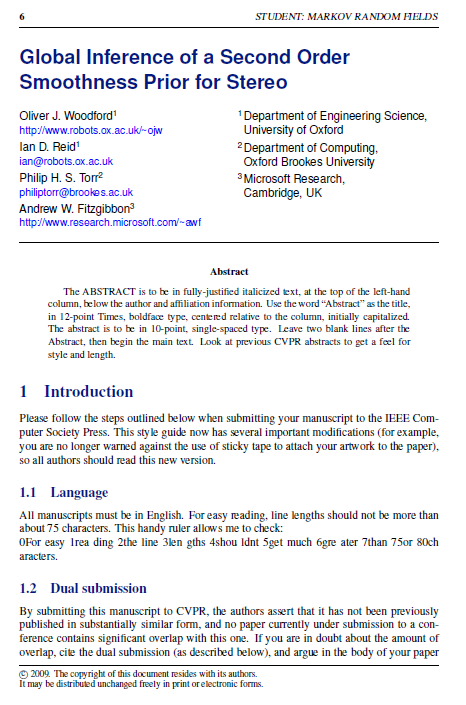
\includegraphics[width=10cm]{images/eg1_largeprint.png}
 \caption{It is often a good idea for the first figure to attempt to
 encapsulate the article, complementing the abstract.  This figure illustrates
 the various print and on-screen layouts for which this paper format has
 been optimized: (a) traditional print format; (b) on-screen
 single-column format, or large-print paper; (c) full-screen two column, or
 2-up printing. }
\label{fig:teaser}
\end{figure*}
  

\begin{table}
\begin{center}
\begin{tabular}{|l|c|}
\hline
Method & Frobnability \\
\hline\hline
Theirs & Frumpy \\
Yours & Frobbly \\
Ours & Makes one's heart Frob\\
\hline
\end{tabular}
\end{center}
\caption{Results.   Ours is better.}
\end{table}

%------------------------------------------------------------------------- 
\section{Results}
The proposed method is implemented and publicly available at https://github.com/smortezah/Clusico, under GPLv3 license. The machine used for the tests had an 8-core 3.40 GHz Intel\textsuperscript{\scriptsize\textregistered} Core{\scriptsize\texttrademark} i7-6700 CPU with 32 GB RAM.

For the experiments, we have used 30 mitochondrial DNA (mtDNA) sequences from three groups of Actinopterygii (Ray-finned fishes), Chondrichthyes (Cartilaginous fishes) and Mammalia, that can be downloaded from https://www.ncbi.nlm.nih.gov/nuccore. The size of these sequences varies from 16,189 to 18,431 bases.

In order to classify the sequences, we first ran GeCo on all sequences, considering them as references as well as targets. As the result, normalized relative compression (NRC) values were obtained, that can be calculated as


\bibliography{ref}
\end{document}
